
%----------------------------------------------------------------------------------------
%	PACKAGES AND DOCUMENT CONFIGURATIONS
%----------------------------------------------------------------------------------------

\documentclass[a4paper]{article} %Article class
\usepackage[utf8]{inputenc} %utf-8 Encoding
\usepackage{graphicx} % Required for the inclusion of images
\usepackage{float} %requiered for image positioning
\graphicspath{{Figures/}} % Set the default folder for images
\usepackage{amsmath} % Required for some math elements 
\usepackage[english]{babel} % Language 
\setlength\parindent{0pt} % Removes all indentation from paragraphs
\usepackage{xcolor}	
\usepackage{listings} %Requiered for code inclusion
\renewcommand{\labelenumi}{\alph{enumi}.} % Make numbering in the enumerate environment by letter rather than number (e.g. section 6)
\usepackage[
backend=biber,
style=alphabetic,
sorting=ynt
]{biblatex}
\addbibresource{sample.bib}

\usepackage{color}
\lstset{ %
	language=R,                     % the language of the code
	basicstyle=\footnotesize,       % the size of the fonts that are used for the code
	numbers=left,                   % where to put the line-numbers
	numberstyle=\tiny\color{gray},  % the style that is used for the line-numbers
	stepnumber=1,                   % the step between two line-numbers. If it's 1, each line
	% will be numbered
	numbersep=5pt,                  % how far the line-numbers are from the code
	backgroundcolor=\color{white},  % choose the background color. You must add \usepackage{color}
	showspaces=false,               % show spaces adding particular underscores
	showstringspaces=false,         % underline spaces within strings
	showtabs=false,                 % show tabs within strings adding particular underscores
	frame=single,                   % adds a frame around the code
	rulecolor=\color{black},        % if not set, the frame-color may be changed on line-breaks within not-black text (e.g. commens (green here))
	tabsize=2,                      % sets default tabsize to 2 spaces
	captionpos=b,                   % sets the caption-position to bottom
	breaklines=true,                % sets automatic line breaking
	breakatwhitespace=false,        % sets if automatic breaks should only happen at whitespace
	title=\lstname,                 % show the filename of files included with \lstinputlisting;
	% also try caption instead of title
	keywordstyle=\color{blue},      % keyword style
	commentstyle=\color{dkgreen},   % comment style
	stringstyle=\color{mauve},      % string literal style
	escapeinside={\%*}{*)},         % if you want to add a comment within your code
	morekeywords={*,...},
	% if you want to add more keywords to the set
	alsoletter={.}        % if you want to add more keywords to the set
} 


%----------------------------------------------------------------------------------------
%	DOCUMENT INFORMATION
%----------------------------------------------------------------------------------------

\title{Network Intruder Detection \\
\large APA Practical Work \\
Universitat Politècnica de Catalunya} % Title
\author{Lluc Bové \& Aleix Trasserra} % Author name

\date{Q1 2016-17}

\begin{document}

\maketitle % Insert the title, author and date


%----------------------------------------------------------------------------------------
%	INTRO
%----------------------------------------------------------------------------------------

\section{Introduction}
In the area of \textit{computer security}, one of the current works is to protect computer networks from unauthorized users. \\
The goal of this work is to build a system capable of predicting if a connection is an \textit{intrusion} (and what kind of intrusion) or if it is a normal connection. 
 
\subsection{The data}
Our dataset\footnote{The original dataset can be obtained visiting the following link:\\  http://kdd.ics.uci.edu/databases/kddcup99/kddcup99.html} is a set of \textbf{connection records}.
A \textbf{connection} is a set of TCP packets starting and ending at some well defined times, between which data flows from a \textit{source IP} address to a \textit{target IP} address under some well defined \textit{protocol}.
There are four main attack categories that our system will classify other than \textit{normal connections}:
\begin{itemize}
	\item DOS: denial-of-service.
	\item R2L: unauthorized access from a remote machine.
	\item U2R: unauthorized access to local superuser(root) privileges.
	\item probing: surveillance and other probing, e.g: port scanning.
\end{itemize}


%----------------------------------------------------------------------------------------
%	Related
%----------------------------------------------------------------------------------------

\section{Related Work}
The paper \textit{Cost-based Modeling and Evaluation for Data Mining With Application to Fraud and Intrusion Detection Results from the JAM Project by Salvatore J. Stolfo, Wei Fun, Wenke Lee, Andreas Prodromids and Philip`K. Chan.} from the Florida Institute of Technology talks about JAM project. \\
The paper describes the results achieved using a JAM distributed data mining system for the problem of fraud detection in financial information systems. \\

Other work related with \textit{network intrussion} problem was reported by Ramesh Agarwal and Mahesh V. Joshi. They described a rule called \textit{PN-rule} which is a framework for learning classifier models and its study case was network intrusion detection.
%----------------------------------------------------------------------------------------
%	Data exploration
%----------------------------------------------------------------------------------------

\section{Data Exploration Process}
In this section we will take a first look to our data, in order to know what are we going to analyse. First we'll preprocess it, this includes detecting outliers, missing values... And deleting them. Then we are going to perform a feature extraction and selection. This consists in deleting variables that aren't necessary and deriving new ones. Then we'll visualize our data using FDA and finally we'll do a clustering. All this process can be followed using the script provided called \textit{dataExploration.R}.\\

\subsection{Preprocessing}
The original data has two forms. The first one has a dimension of 5 million rows approximately and the other is a reduction of 10\%. We assured that this purge didn't affect the proportion of less used attack types, and it didn't, so from now on we will work with this reduction.\\

First of all when we analyse our dataset we see that variables have no name, so we name them. Then we execute \lstinline|summary| to detect abnormal things on our data, like strange means, medians, extreme values, errors... So we first realize that our categorical variables aren't factors, and they have no text. To solve this first we declare all categorical as factors and we use \lstinline|TRUE| and \lstinline|FALSE| for boolean ones, and we use names for the others. We realize that some variables do not vary so we delete them. We detected an error with a boolean factor, it had missing values so we deleted the rows.


\subsection{Feature extraction/selection}
First we need to define the target variable. We decide to use the main attack in the network. This is a category for each attack type. The variable is defined as table \ref{table:main} shows. 
\begin{table}
	\begin{tabular}{ll}
		Main Attack & Attack Type                                                            \\ \hline
		DOS         & back, land, neptune, smurf, teardrop                                       \\
		U2R         & buffer overflow, loadmodule, perl, rootkit                               \\
		R2L         & ftp\_write, guess password, imap, multihop, phf, spy, warezclient, warezmaster \\
		probe       & ipsweep, nmap, portsweep, satan                                           \\
		normal      & normal                                                                 \\
	\end{tabular}
	\caption{This table shows the main attack classification}
	\label{table:main}
	
\end{table}
Now we have this categorization so we don't need attack type any more but we save it because it may be a useful alternative target respect main attack. 


\subsection{Descriptive Analysis}
We'll proceed to do a descriptive analysis of our data. To make our graphs more beautiful we use \textit{ggplot2}\cite{ggplot}. For every numerical variable we do a histogram and a boxplot. We realize that the median of many variables is 0, that is, half of the data is zero. This is because some variables are TCP camps that hardly ever are used but when are used they are important. Another cause is that many variables depend on if the communication is between the host and the server or the server and the host. This is why we want to show this variables without including the zero's. We also applied a $log$ transformation. Now we will show some of this plots:\\

\begin{figure}[H]
	\centering
	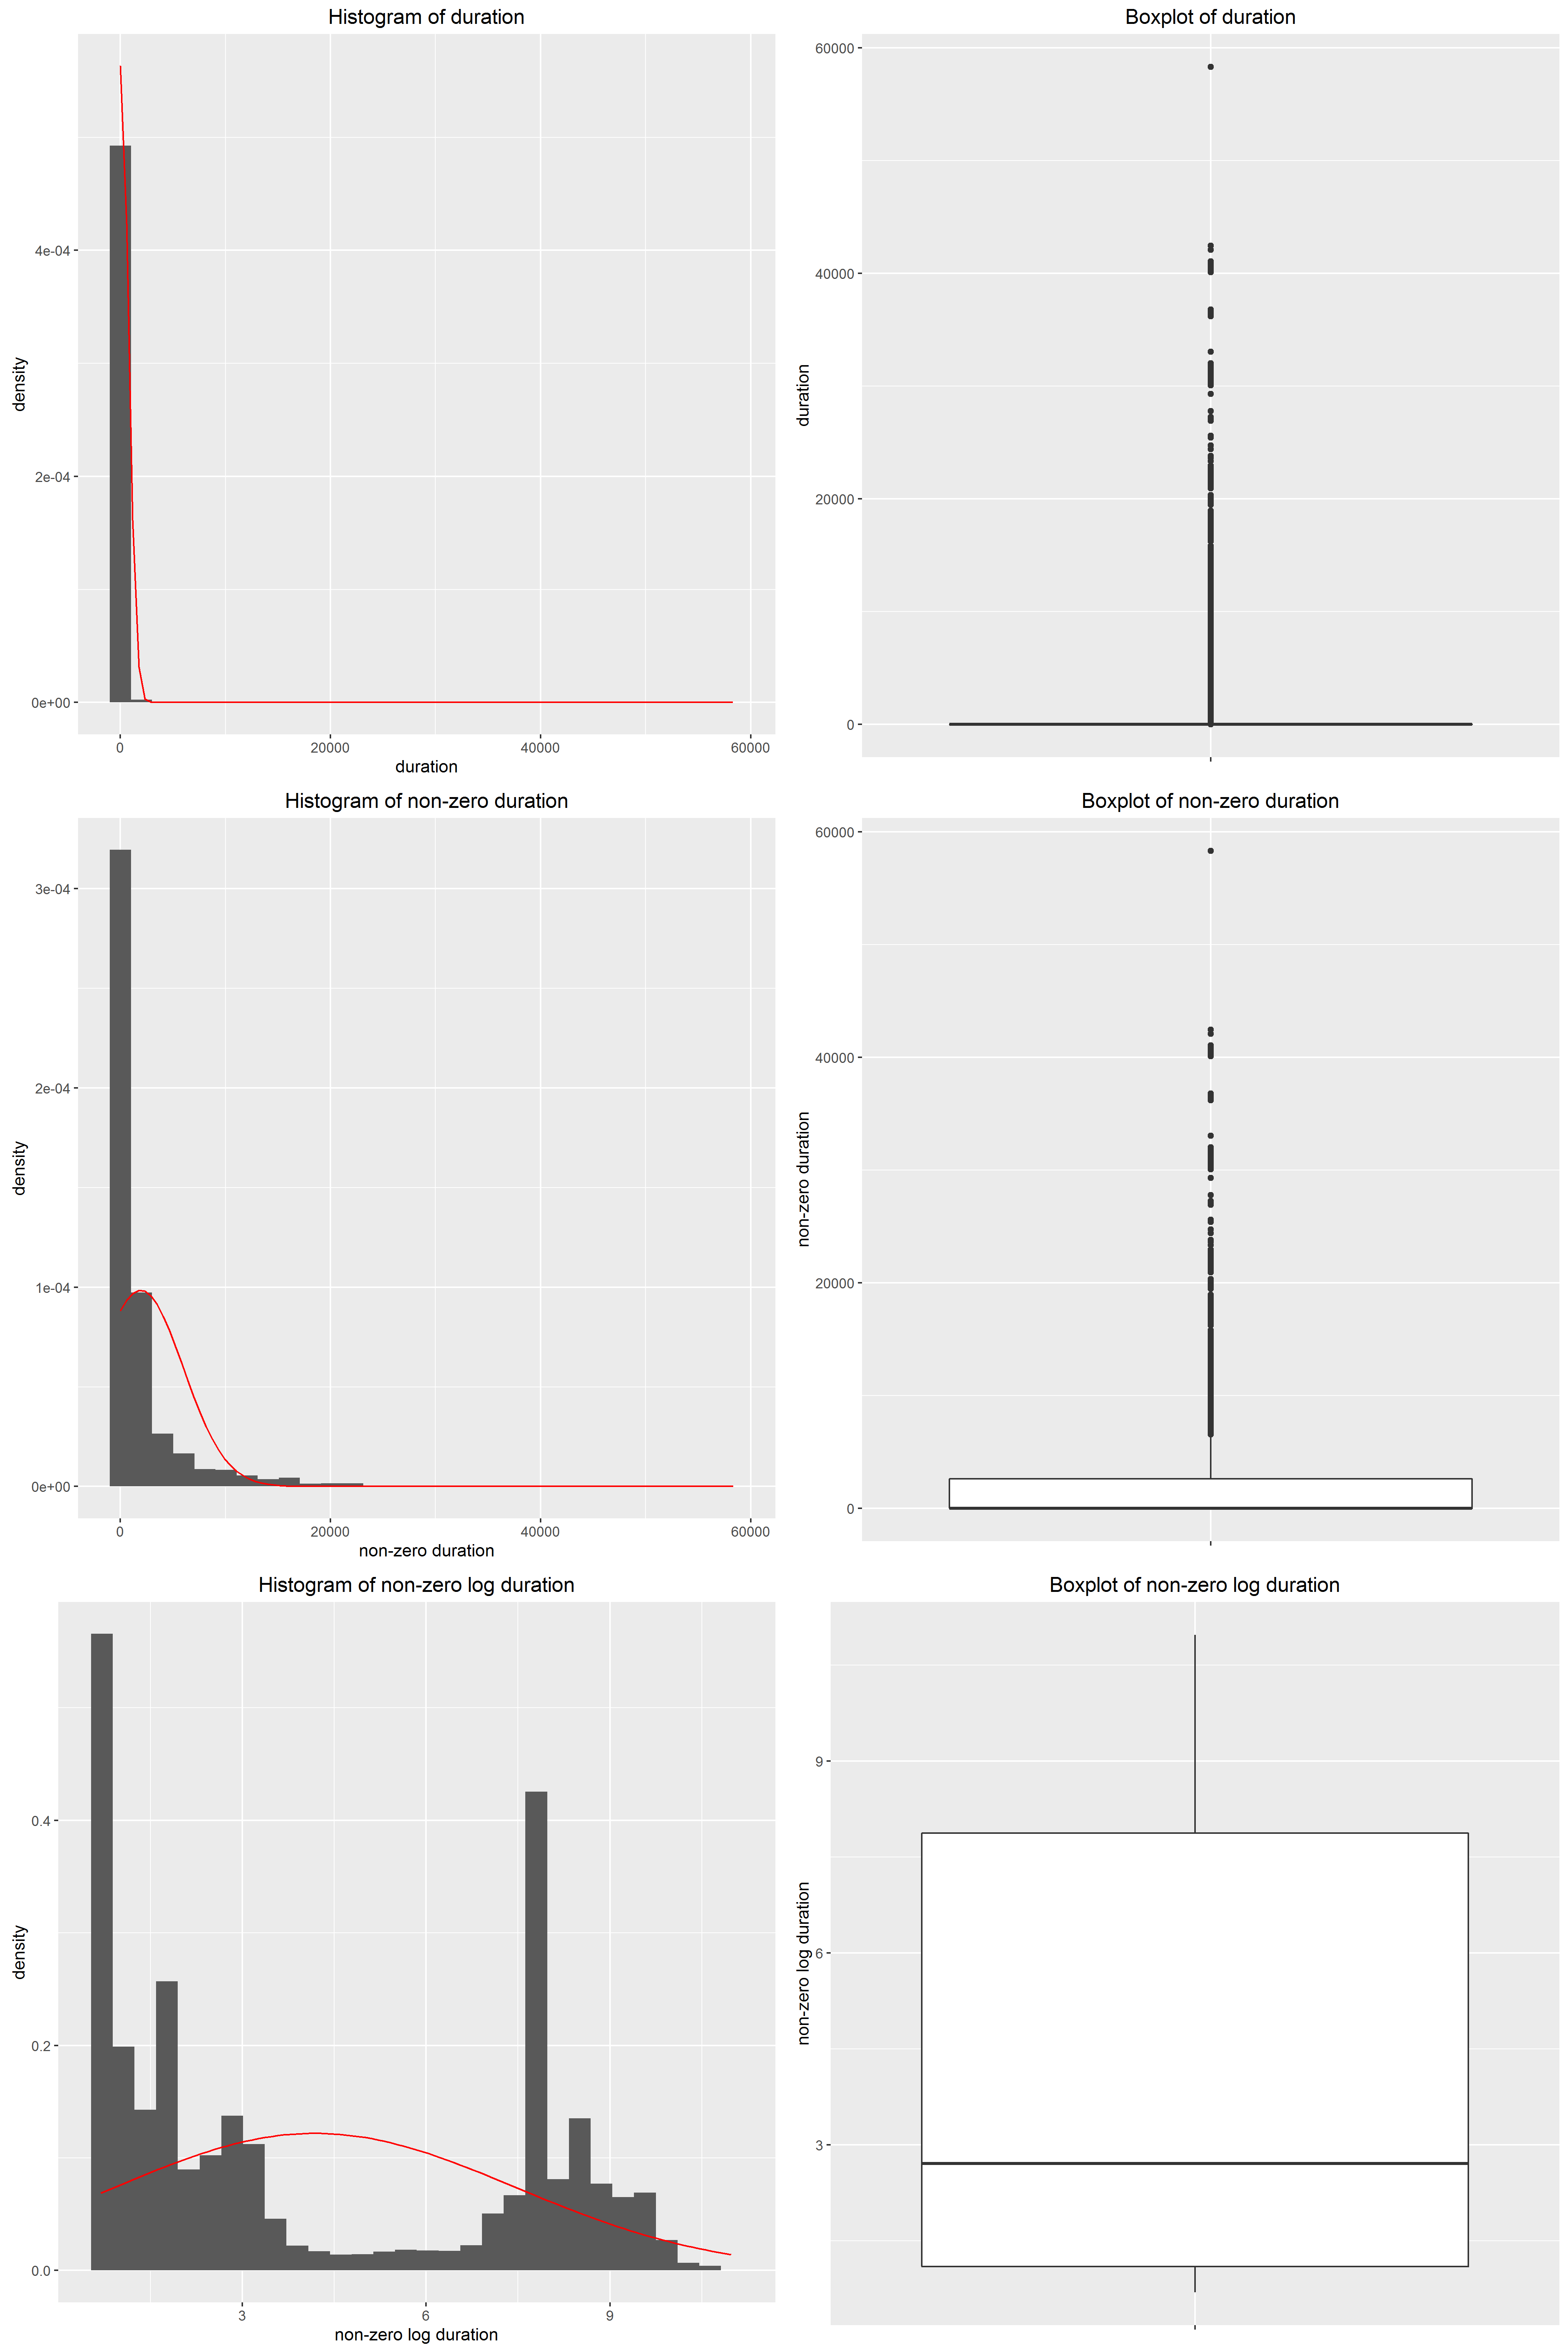
\includegraphics[scale=0.25]{duration.png}
	\caption{This figure shows descriptive graphs for the duration variable}
	\label{fig:duration}
\end{figure}

Figure \ref{fig:duration} shows the boxplot and histogram for the variable \textit{duration}, that is the duration of the TCP connection. We can see that most TCP connections have a duration lower than zero. This causes that histogram and boxplot are difficult to visualize. If we don't display the zero's we fix this. This variable also is advantaged by a $log$ transformation. \\

Many variables have the same structure as the ones before so we don't include them in this analysis. The next thing that we'll do is the descriptive analysis plots for the qualitative variables. We analyse them using contingency tables and bar plots.

Figure \ref{fig:barplots} shows a barplot for main attack variable. We want to emphasize that it has an unequal distribution. Most connections are DOS attacks, followed by normal and then probe. R2L and U2L are in a tiny proportion.

\begin{figure}[H]
	\centering
	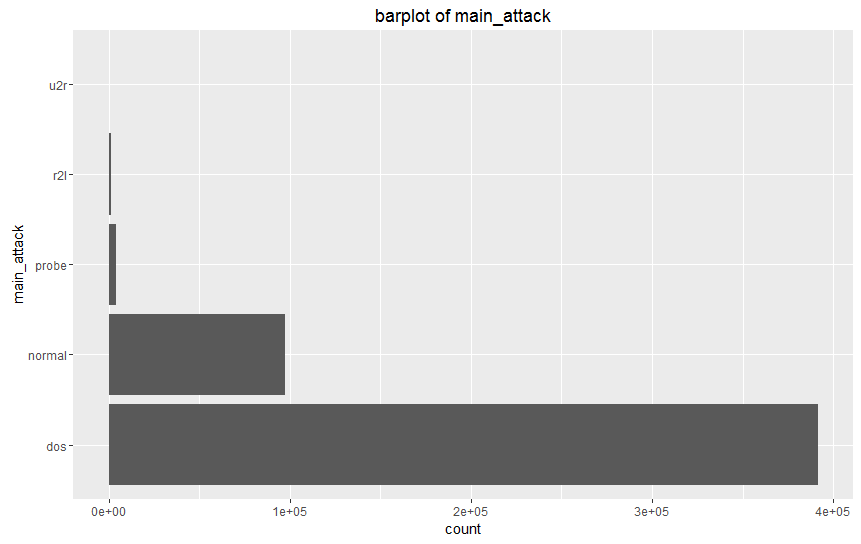
\includegraphics[scale=0.5]{bar_main_attack.png}
	\caption{Barplot for main attack}
	\label{fig:barplots}
\end{figure}
We made contingency tables from some of the most relevant variables, against the main attack variable. This variables are protocol, flags, service and superuser attempted. Figure \ref{fig:cont} shows the result. 

\begin{figure}[H]
	\centering
	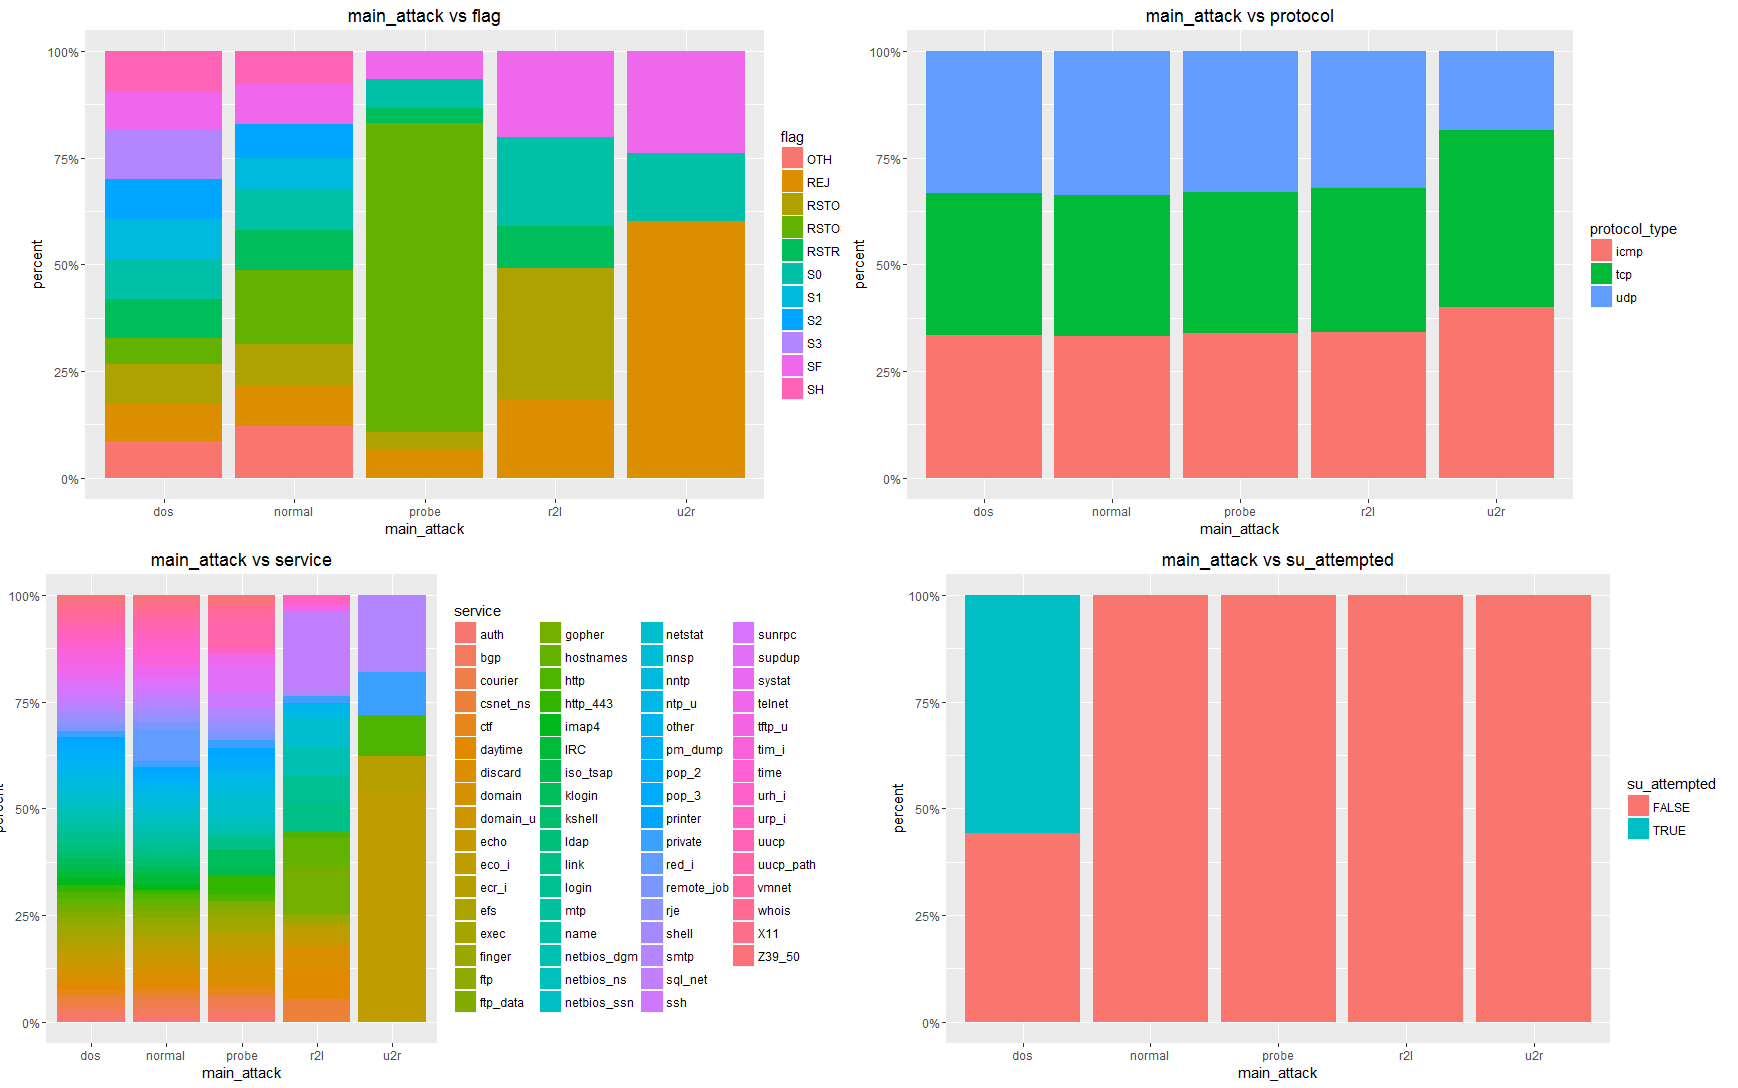
\includegraphics[scale=0.85]{cont.png}
	\caption{Contingency tables represented }
	\label{fig:cont}
\end{figure}

We can observe that for example, DOS attacks and normal connections have similar flags, in probe attacks the flag \textit{RESET} is very often, and in \textit{U2R} it predominates \textit{REJ}. In all types of connections the protocols used are similar. The services are almost the same with normal connections, DOS and PROBE attacks. They differ with the R2L and U2L attacks and the service that predominates in U2L is \textit{eco\_i}. The only tpye of connection that does request super user is DOS attacks.
\subsection{Visualization}
To do visualization we use the Fisher Discriminant Analysis or FDA. We apply it using only numerical variables and our classes are the different values of main attack. The visualization of the first two components can be observed in figure \ref{fig:fda}.

\begin{figure}[H]
	\centering
	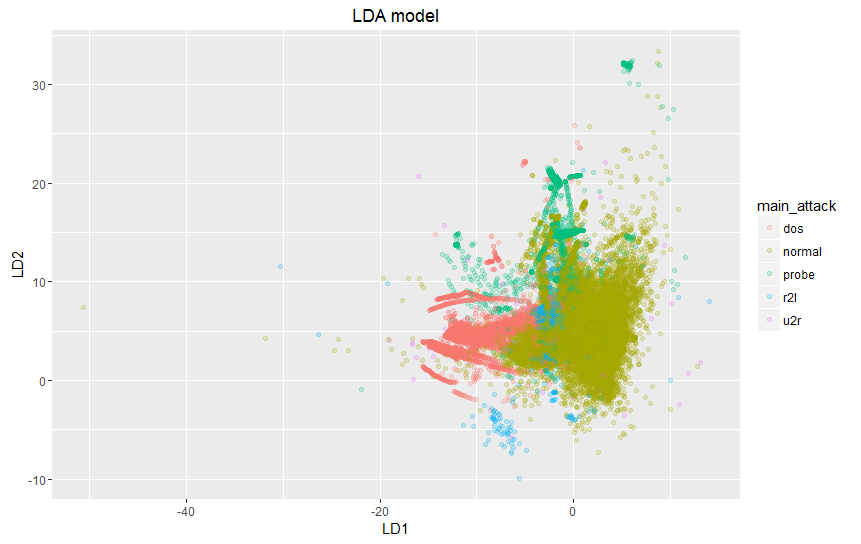
\includegraphics[scale=0.45]{LDA.png}
	\caption{LDA visualization}
	\label{fig:fda}
\end{figure}

The classes don't seem very separated. In fact, if we didn't use colours we wouldn't have seen the classes separated. This indicates us that the prediction task can be a big challenge. The trace of the two first components sum 98.49\%.




%----------------------------------------------------------------------------------------
%	Classification
%----------------------------------------------------------------------------------------

\section{Classification}
\subsection{Linear Methods}
\subsubsection{Logistic regression}
In this section we will show our experiments done using logistic regression. \\
Logistic regression must be trained with a binary classification so we transformed our data, so that the target variable classification will be \textit{normal connection} or \textit{attack}.

First of all, we'll train a model using \textit{logistic regression} with our original dataset, which we know that is unbalanced.
We also used the AIC index in order to simplify the model.\\
We use \textit{P} to denote the cut value of the logistic regression.
With our trained model we'll try which value of \textit{P} gives us better results, keeping in mind that we prefer a normal connection to be detected as an attack(false positive) rather than an attack predicted as a normal connection (false negative)  \\
We tried different values of P in the range of (0.4,0.7) in steps of 0.1.
\begin{table}[h]
	\centering
	\begin{tabular}{l|llll}
		P              & 0.4  & 0.5   & 0.6   & 0.7   \\
		\hline 
		Training error & 30.4 & 30.46 & 30.54 & 30.63 \\
		Test error     & 7.67 & 7.71  & 7.75  & 7.79 
	\end{tabular}
	\caption{Train and test errors depending on P}
	\label{cut}
\end{table}

If we observe the values in table\ref{cut}, for P=0.4 the test and training error are the best ones. \\

We observe the confusion matrix in order to analyse the classification more deeply.

\begin{table}[h]
	\centering
	\begin{tabular}{l|ll}
		& Pred   &        \\
		Truth  &        &        \\
		& normal & attack \\
		\hline
		normal & 59526  & 1063   \\
		attack & 22790  & 227646
	\end{tabular}
	\caption{Confusion matrix of logistic regression model with P = 0.4}
	\label{logistic}
\end{table}

In table \ref{logistic} we can observe that the false-positive rate is 9.10\% and the true-positive rate is 1.75\%  . \\
We observe that logistic regression works better when we give higher relevance to attack connections.

\subsubsection{Multinomial regression}
We tried to apply a multinomial regression to our data. We knew that our data is unbalanced but we first tried to train the classifier without treating the data. We get a training error of 0.05\%, and a test error of 7.79\%,. Although the test error percentage is low the minority classes like \textit{U2R} or \textit{R2L} are badly generalized, as table \ref{table:unbModel} shows. A high percentage of \textit{U2R} attacks are miss-predicted, and they are the most dangerous ones. Furthermore, they are mostly predicted as normal connections so it would be probable that the attack would stay unnoticed until it would be too late. 

\begin{table}[H]
	\centering
	\begin{tabular}{c | c c c c c}
		& Prediction\\
		Truth\\
		 & Normal & DOS & Probe & R2L & U2R \\
		\hline
		Normal	& 59511	& 95 	 & 953	 & 16 	& 14 \\
		DOS		& 5925	& 223563 & 135	 & 0  	& 807\\
		Probe	& 625	& 163	 & 3125	 & 253	& 0 \\
		R2L		& 15588	& 0		 & 8   & 568 	& 25\\
		U2R		& 190	& 0		 & 0    & 11 	& 27\\	
	\end{tabular}
	\caption{Contingency table of the model that uses all the data}
	\label{table:unbModel}
\end{table}


One solution for unbalanced datasets is to undersample the biggest classes. We tried this solution, we used a balanced but reduced dataset. Then we applied regularization and determined the constant $\lambda$ and the data samples with 10-cross-validation. To do regularization we use the \textit{glmnet} package\cite{glmnet}. The training error for this model is 1.85\% and the test error is 8.06\%.


\begin{table}[H]
	\centering
	\begin{tabular}{c | c c c c c}
			& Prediction\\
		Truth\\
				& Normal & DOS & Probe & R2L & U2R \\
		\hline
		Normal	& 59055	& 66 	 & 539	 & 122 	& 807 \\
		DOS		& 7349	& 222221 & 225	 & 0  	& 58\\
		Probe	& 229	& 50	 & 3857	 & 0	& 30 \\
		R2L		& 14838	& 1		 & 305   & 688 	& 357\\
		U2R		& 79	& 0		 & 35    & 1 	& 113\\	
	\end{tabular}
	\caption{Contingency table of the under-sampled regularized 10CV multinomial model}
	\label{table:sub10model}
\end{table}

Table \ref{table:sub10model} shows the contingency table of the model. The horizontal header is the model prediction and the vertical one is the real classification. Test dataset is used in order to produce this table so the results show how well generalizes the model. Although test error is worse in than the unbalanced model, predictions of the less populated classes are more accurate, in general. We observe that 28\% of the connections that are predicted as normal ones are indeed network attacks, so the number of false negatives is quite big and most of them are of \textit{R2L} which is a dangerous attack. Nevertheless a little proportion of \textit{U2R} attacks are miss-predicted as normal connections. 

%\subsection{Non Linear Methods}


%----------------------------------------------------------------------------------------
%	BIBLIOGRAPHY
%----------------------------------------------------------------------------------------
\nocite{*}
\printbibliography

%----------------------------------------------------------------------------------------


\end{document}